\documentclass{hw_template}

\usepackage{arydshln}

\title{\bfseries Іспит з Біомеханіки}
\author{\bfseries Захаров Дмитро}
\date{16 грудня, 2024}

\begin{document}

\pagestyle{fancy}

\maketitle

\tableofcontents

\vspace{10px}

\section{Теоретичне Питання}

\begin{problems}
    Напрямки сучасної біомеханіки: 5-6 прикладів.
\end{problems}

\textbf{Відповідь.} Сучасна біомеханіка --- це в першу чергу міждисциплінарна
наука, що поєднує в собі безліч технічних та біологічних галузей: фізика
(термодинаміка, механіка, електродинаміка, фізика течії та навіть теорію
електричних кіл (реологічні моделі тощо)), комп'ютерні науки (обробка даних,
нейронні мережі для аналізу зображень та відео), математика (диференціальні
рівняння, теорія ймовірностей, моделювання, статистика), біологія (генетика,
анатомія тощо). Через це, сучасна біомеханіка включає в себе безліч напрямків,
котрі так чи інакше поєднують у собі ці галузі. Розглянемо деякі з них:
\begin{itemize}
    \item \textbf{Біомеханіка Руху Людини}/\textbf{Спортивна біомехінка}.
    Включає в собі вивчення ходьби, бігу, спортивних рухів для покращення
    продуктивності спорстменів або реабілітації пацієнтів (кінезіологія).
    Створення алгоритмів для аналізу кінематики та кінетики рухів. Зокрема,
    деякі з них використовуються для розробки відеоігор, або для аналізу рухів у
    фізіотерапії.
    \item \textbf{Nature-Inspired Біомеханіка}. Вивчення природних об'єктів для
    створення нових технологій. Наприклад, дуже актуальним напрямком в рамках
    повномасштабного вторгнення Росії в Україну є Swarm Intelligence для
    розробки управління системою дронів. 
    \item \textbf{Біоніка.} Напрямок, що вивчає природні системи та механізми 
    з метою створення інженерних рішень, технологій або пристроїв, які наслідують 
    принципи природи. Відомий приклад --- роботи-собаки від Boston Dynamics, що
    досліджують природу руху тварин для того, щоб відтворити ці рухи у роботах. Так
    само, можна навести приклад комп'ютерних вірусів, що моделюють розповсюдження
    вірусів у природі, радіочастотна ідентифікація (RFID), що пішла від синіх 
    метеликів Морфо тощо. 
    \item \textbf{Ергономіка.} Досліджує взаємодію людини з робочим середовищем,
    інструментами та обладнанням з метою відвищення комфорту, продуктивності 
    та безпеки. Включає, наприклад, фізичну ергономіку, що оцінює дизайн 
    крісел для запобігання болю у спині чи регульованих столів для роботи стоячи.
    Також, можна виділити когнітивну ергономіку, що вивчає процеси мислення,
    прийняття рішень для створення комфортного інформаційного середовища (зрозумілі 
    інтерфейси у смартфонах чи автомобілях).
    \item \textbf{Медична біомеханіка.} Досліджує механічні властивості та
    процеси у людському тілі, щоб зрозуміти фізичну взаємодію між різними його
    структурами та допомогти у лікуванні й розробці медичних пристроїв. Як приклад 
    можна навести кардіоваскулярну біомеханіку, що вивчає механіку кровотоку 
    та функцію серця і судин (розробка штучних сердечних клапанів і стентів/моделювання
    гемодинаміки для діагностики аневризми). Також існує нейробіомеханіка, що
    досліджує взаємодію механічних і нервових систем (розробка екзоскелетів для
    пацієнтів з ураженим спинним мозком), або ж стоматологічна біомеханіка (зубні 
    імпланти) тощо.
    \item \textbf{Оптимальні біомеханічні системи.} Структури та механізми в
    природі сформувалися в результаті еволюційного відбору, щоб забезпечити
    максимальну ефективність функціонування при мінімальних енергетичних
    затратах. Саме тому нам цікаво адаптаптувати технології та рішення з природи
    для створення оптимальних біомеханічних систем. Наприклад, кістки мають
    легку, але міцну будову завдяки комбінації щільної зовнішньої кори та
    пористої внутрішньої структури, що можна використати у створенні легких
    конструкцій для авіації чи автомобілебудування. Риби мають гідродинамічну
    форму тіла та хвилеподібний рух, що мінімізують загальний опір у воді, що
    можна використати при розробці маневрених та швидких підводних апаратів. 
\end{itemize}

\section{Теорія Розмірності}

\begin{problems}
    Відповісти на наступні запитання:
    \begin{enumerate}[(A)]
        \item Получить выражение для безразмерного критерия подобия, который зависит от частоты колебаний $\nu$, характерного размера $\ell$ и скорости $v$.
        \item Получить выражение для потенциальной энергии $W_p$, если известно, что она зависит от массы тела $m$, высоты $h$ и ускорения свободного падения $g$. Проанализировать все возможные случаи с учетом каждого из Пи-параметров.
    \end{enumerate}
\end{problems}

\textbf{Відповідь.}

\textbf{Пункт (А).} Отже, маємо безрозмірну величину $k = k(\nu,\ell,v)$.
Відповідь можна дати одразу, згадавши курс шкільної фізики: величина $2\pi\nu
\ell$ відповідає лінійній швидкості обертального руху з частотою (не циклічною)
$\nu$ та радіусом $\ell$. Тому, відношення $(\nu \ell/v)^{\alpha}$ для
будь-якого $\alpha$ дасть безрозмірну величину. Проте, оскільки ми завжди можемо
зробити заміну $\widetilde{k} := k^{1/\alpha}$, то можемо без обмеження
загальності взяти найпростіше відношення $\nu \ell/v$ як безрозмірний критерій.

Отримаємо це методом розмірності. Нехай $k=\nu^{\alpha}\ell^{\beta}v^{\gamma}$.
Розпишемо розмірності. Нехай $L$ --- відстань (метри), $T$ --- час (секунди).
Тоді:
\begin{equation*}
    [k] = T^{-\alpha} \times L^{\beta} \times L^{\gamma}T^{-\gamma} = T^{-\alpha-\gamma}L^{\beta+\gamma}.
\end{equation*}

Звідси $\gamma=-\alpha$ та $\beta=\alpha$, тому
$k=\nu^{\alpha}\ell^{\alpha}v^{-\alpha} = (\nu\ell/v)^{\alpha}$. Отже,
безрозмірний критерій подібності --- $k(\nu,\ell,v) = \nu\ell/v$.

\textbf{Пункт (Б).} Потенціальна енергія має вигляд $W_p = W_p(m,h,g)f(\Pi)$. Знову ж таки,
доволі нескладно згадати шкільну формулу $W_p=mgh$. Виведемо це формально. Енергія 
вимірюється у Джоулях, або добуток сили на відстань. Оскільки сила має розмірність $M/(L \times T^2)$, де
$M$ --- маса, $L$ --- відстань, $T$ --- час, то потенціальна енергія має розмірність $M \times L^2/T^2$.
Якщо вважаємо $W_p=m^{\alpha}h^{\beta}g^{\gamma}$, то маємо:
\begin{equation*}
    [W_p] = M^{\alpha} \times L^{\beta} \times L^{\gamma}T^{-2\gamma} = ML^2T^{-2}
\end{equation*} 

Звідси маємо систему рівнянь:
\begin{equation*}
    \begin{cases}
        \alpha = 1, \\
        \beta + \gamma = 2 \\
        -2\gamma = -2.
    \end{cases}
\end{equation*}

Звідси $(\alpha,\beta,\gamma) = (1,1,1)$, себто $W_p=mgh \times f(\Pi)$. 

Залишилось проаналізувати $\Pi$-параметри. Чи можемо ми, скомбінувавши щось з $m,h,g$,
отримати щось безрозмірне? Ні, не можемо. Чому? Оскільки ми маємо три механічні
величини: час, відстань та масу, то кожну ми хочемо отримати з нульовою степінню. 
З величин $m,h,g$ тільки $m$ містить масу, тому $m$ входить з нульовою степенню.
Аналогічно, тільки $h$ містить відстань, а тільки $g$ --- час. Отже, $\Pi$-параметр
не залежить від жодного з параметрів. Таким чином, $W_p=\kappa mgh$, $\kappa \in \mathbb{R}$.

\textbf{Відповідь.} (А) $k = \nu\ell/v$. (Б) $W_p = \kappa mgh$; $\Pi$-параметр не залежить від $m,g,h$.

\newpage

\section{Реологічне співвідношення}
\begin{problems}
    Отримати реологічне співвідношення для наведеної моделі. Провести з нею
ізометричний, ізотонічний та динамічний ($\varepsilon \equiv \varepsilon^*, \sigma \equiv
\sigma^*, \sigma(t) = \exp (i\omega t)$) експерименти; навести графіки
динамічної поведінки (навантаження і релаксація) $\varepsilon(t)$ і $\sigma(t)$
для відповідних ступінчатих навантажень $\varepsilon^*(t), \varepsilon^{**}(t)$
і $\sigma^*(t), \sigma^{**}(t)$, а також формули для дійсної (амплітуда) та
уявної (фазовий зсув) частин у випадку динамічного експерименту. Наведена модель
– це в’язкопружна рідина або твердий біологічний матеріал?
\begin{center}
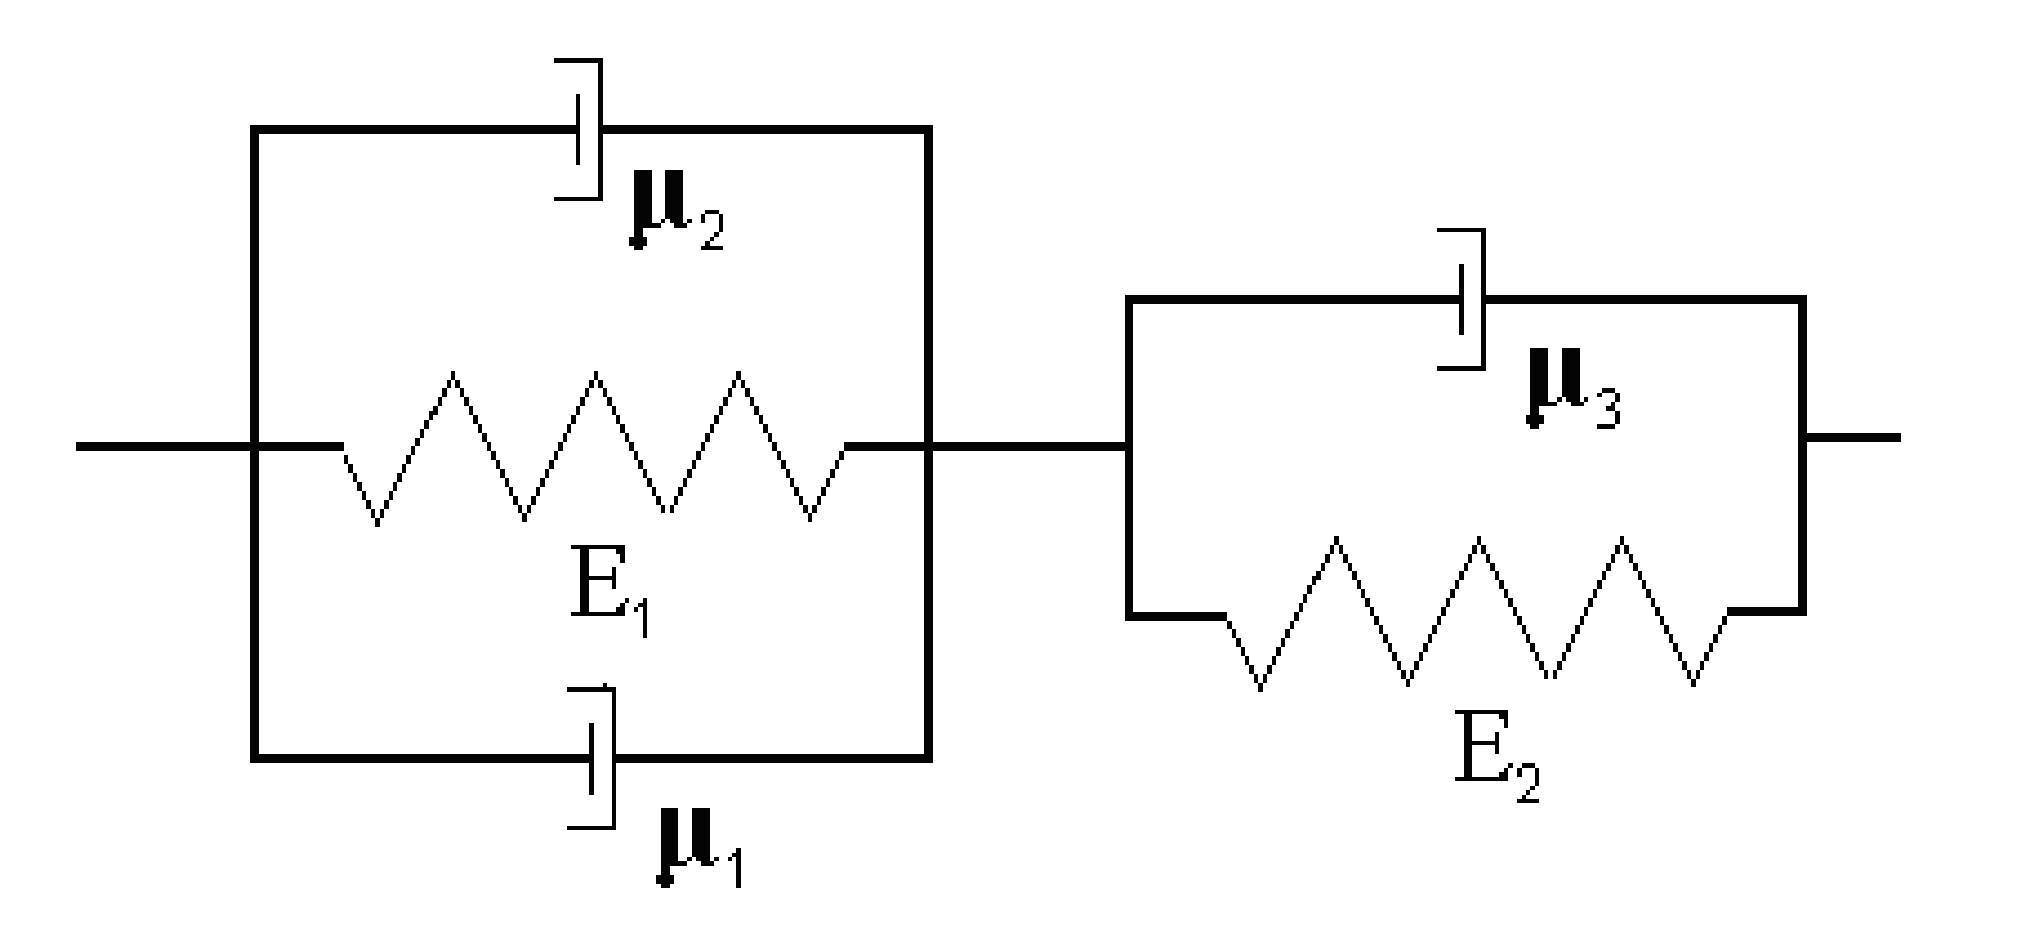
\includegraphics[width=0.5\textwidth]{images/exam/problem.png}
\end{center}
\end{problems}

\textbf{Розв'язання.} 

\textcolor{blue!90!white}{\textbf{Частина 1. Система рівнянь.}} Згадаємо, що
реологічне співвідношення для еластичних тіл $\sigma =
E\varepsilon$ для малих деформацій, де $E$ – модуль Юнга. Для
в'язкої рідини формула Ньютона: $\sigma = \mu \dot{\varepsilon}$, де $\mu$ –
коефіцієнт в'язкості. 

Тепер, виведемо рівняння, що описує динаміку в описаній системі. Помітимо, що
при послідовному з'єднанні, напруга в кожному елементі однакова, а деформація
є сумою деформацій в кожному елементі. При паралельному з'єднанні, деформація
в кожному елементі однакова, а напруга є сумою напруг в кожному елементі. 

Таким чином, позначимо розтягнення перших трьох елементів як $\varepsilon_1$, а
останніх двох – $\varepsilon_2$, таким чином $\varepsilon = \varepsilon_1 +
\varepsilon_2$. Розглянемо першу групу елементів. Для середнього елементу 
$\sigma_2 = E_1\varepsilon_1$. Для першого і третього елементів маємо
$\sigma_1 = \mu_1 \dot{\varepsilon}_1$ та $\sigma_3 = \mu_2 \dot{\varepsilon}_1$.
Окрім того, оскільки з'єднання паралельне, то $\sigma = \sigma_1 + \sigma_2 + \sigma_3$.

Тепер, розглянемо другу групу елементів. Для верхнього елементу маємо
$\sigma_4 = \mu_3\dot{\varepsilon}_2$ і, нарешті, для нижнього 
$\sigma_5 = E_2 \varepsilon_2$. Оскільки з'єднання паралельне, то 
$\sigma = \sigma_4 + \sigma_5$.

Випишемо усі рівняння разом:
\begin{equation*}
    \begin{cases}
        \varepsilon = \varepsilon_1 + \varepsilon_2, \\
        \sigma = \sigma_1 + \sigma_2 + \sigma_3 = \sigma_4 + \sigma_5, \\
        \sigma_1 = \mu_1 \dot{\varepsilon}_1, \sigma_2 = E_1 \varepsilon_1,\\
        \sigma_3 = \mu_2 \dot{\varepsilon}_1, \sigma_4 = \mu_3 \dot{\varepsilon}_2, \sigma_5 = E_2 \varepsilon_2.
    \end{cases}
\end{equation*}

Залишилося їх об'єднати в одне велике диференціальне рівняння. 

\textcolor{blue!90!white}{\textbf{Частина 2. Зведення до одного рівняння.}} Підставимо 
усі напруги у рівність для $\sigma$:
\begin{equation*}
    \begin{cases}
        \varepsilon = \varepsilon_1 + \varepsilon_2, \\
        \sigma = (\mu_1+\mu_2)\dot{\varepsilon}_1 + E_1\varepsilon_1, \\
        \sigma = \mu_3\dot{\varepsilon}_2 + E_2\varepsilon_2.
    \end{cases}
\end{equation*}

Скористаємося методом операторів. Введемо два оператори:
\begin{equation*}
    \Gamma_1 := (\mu_1+\mu_2)\frac{d}{dt} + E_1, \quad \Gamma_2 := \mu_3\frac{d}{dt} + E_2.
\end{equation*}

В такому разі, система рівнянь може бути записана у вигляді:
\begin{equation*}
    \begin{cases}
        \varepsilon = \varepsilon_1 + \varepsilon_2, \\
        \sigma = \Gamma_1\varepsilon_1, \\
        \sigma = \Gamma_2\varepsilon_2.
    \end{cases}
\end{equation*}

Звідси, $\varepsilon_1 = \Gamma_1^{-1}\sigma$, $\varepsilon_2 =
\Gamma_2^{-1}\sigma$, отже $\varepsilon = \Gamma_1^{-1}\sigma +
\Gamma_2^{-1}\sigma$. Помножимо обидва боки на $\Gamma_1\Gamma_2$:
\begin{equation*}
    \Gamma_1\Gamma_2\varepsilon = (\Gamma_1 + \Gamma_2)\sigma.
\end{equation*}

Далі достатньо лише підставити оператори:
\begin{equation*}
    \textcolor{blue!90!white}{(\mu_1+\mu_2)\mu_3\ddot{\varepsilon} + (E_1\mu_3 + E_2(\mu_1+\mu_2))\dot{\varepsilon} + E_1E_2\varepsilon = (E_1 + E_2)\sigma + \left(\mu_1+\mu_2+\mu_3\right)\dot{\sigma}}
\end{equation*}

Перейдемо до експериментів.

\textcolor{blue!90!white}{\textbf{Частина 3.1. Ізометричний експеримент.}} Для 
ізометричного експерименту маємо $\varepsilon \equiv \varepsilon^*$. Підставляючи,
рівняння стає:
\begin{equation*}
    \frac{d\sigma}{dt} + \frac{E_1 + E_2}{\mu_1+\mu_2+\mu_3}\sigma = \frac{E_1E_2}{\mu_1+\mu_2+\mu_3}\varepsilon^*.
\end{equation*}

Це звичайне лінійне диференціальне рівняння першого порядку. Розв'язуємо однорідну 
частину $\sigma_H(t)$:
\begin{equation*}
    \frac{d\sigma_H}{dt} = -\frac{E_1 + E_2}{\mu_1+\mu_2+\mu_3}\sigma _H
    \implies \frac{d\sigma_H}{\sigma_H} = -\frac{E_1 + E_2}{\sigma_1+\sigma_2+\sigma_3}dt
\end{equation*}

Проінтегрувавши обидві частини, отримаємо:
\begin{equation*}
    \sigma_H(t) = \widetilde{\sigma} \exp\left(-\frac{E_1 + E_2}{\mu_1+\mu_2+\mu_3}t\right).
\end{equation*}

Використовуємо метод варіації стали для пошуку частинного розв'язку. Припустимо,
що $\sigma(t) = \widetilde{\sigma}(t)\exp\left(-\frac{E_1 + E_2}{\mu_1+\mu_2+\mu_3}t\right)$.
Позначимо через $1/T \equiv \frac{E_1 + E_2}{\mu_1+\mu_2+\mu_3}$, тоді $\sigma(t) = \widetilde{\sigma}(t)e^{-t/T}$.
Тоді, підставляючи у рівняння, отримаємо:
\begin{equation*}
    \frac{d\widetilde{\sigma}}{dt}e^{-t/T} - \frac{1}{T}\widetilde{\sigma}e^{-t/T} + \frac{1}{T}\widetilde{\sigma}(t)e^{-t/T} = \frac{E_1E_2}{T(E_1+E_2)}\varepsilon^*
\end{equation*}

І це, очікувано, спрощується до:
\begin{equation*}
    \frac{d\widetilde{\sigma}}{dt}e^{-t/T} = \frac{E_1E_2}{T(E_1+E_2)}\varepsilon^* \implies \frac{d\widetilde{\sigma}}{dt} = \frac{E_1E_2}{T(E_1+E_2)}\varepsilon^*e^{t/T}
\end{equation*}

Інтеруємо обидві частини:
\begin{equation*}
    \widetilde{\sigma}(t) = \frac{E_1E_2}{E_1+E_2}\varepsilon^*e^{t/T} + \sigma_C,
\end{equation*}

де $\sigma_C$ – довільна константа інтегрування. Як бачимо, по розмірності
права частина має вигляд $\widetilde{E}\varepsilon^*$, що дійсно відповідає 
напрузі. Отже остаточно:
\begin{equation*}
    \sigma(t) = \left(\frac{E_1E_2}{E_1+E_2}\varepsilon^*e^{t/T} + \sigma_C\right)\exp\left(-\frac{t}{T}\right) = \frac{E_1E_2}{E_1+E_2}\varepsilon^* + \sigma_Ce^{-t/T}, \quad T = \frac{\mu_1+\mu_2+\mu_3}{E_1+E_2}.
\end{equation*}

Отже $\sigma(t) = \frac{E_1E_2}{E_1+E_2}\varepsilon^* + \sigma_Ce^{-t/T}$. Щоб ми мали $\sigma(0)=\sigma_0$, змістимо константу $\sigma_C$, остаточно 
отримавши \textcolor{blue!90!blue}{$\sigma(t) = \frac{E_1E_2}{E_1+E_2}\varepsilon^* + \left(\sigma_0 - \frac{E_1E_2}{E_1+E_2}\varepsilon^*\right)e^{-t/T}$}.

\textcolor{blue!90!white}{\textbf{Частина 3.2. Ізотонічний експеримент.}} Маємо постійну напругу, себто $\sigma \equiv \sigma^*$. Підставляючи, отримаємо:
\begin{equation*}
    (\mu_1+\mu_2)\mu_3\ddot{\varepsilon} + (E_1\mu_3 + E_2(\mu_1+\mu_2))\dot{\varepsilon} + E_1E_2\varepsilon = (E_1 + E_2)\sigma^*
\end{equation*}

Поділимо обидві частини на $(\mu_1+\mu_2)\mu_3$:
\begin{equation*}
    \ddot{\varepsilon} + \frac{E_1\mu_3 + E_2(\mu_1+\mu_2)}{(\mu_1+\mu_2)\mu_3}\dot{\varepsilon} + \frac{E_1E_2}{(\mu_1+\mu_2)\mu_3}\varepsilon = \frac{E_1 + E_2}{(\mu_1+\mu_2)\mu_3}\sigma^*
\end{equation*}

Позначимо $\alpha := \frac{E_1\mu_3 + E_2(\mu_1+\mu_2)}{2(\mu_1+\mu_2)\mu_3}$, $\beta := \frac{E_1E_2}{(\mu_1+\mu_2)\mu_3}$, $\gamma := \frac{E_1 + E_2}{(\mu_1+\mu_2)\mu_3}\sigma^*$. Тоді рівняння має вигляд:
\begin{equation*}
    \ddot{\varepsilon} + 2\alpha\dot{\varepsilon} + \beta\varepsilon = \gamma.
\end{equation*}

Ідейно, для розв'язку знову розв'язуємо однорідну частину, а далі шукаємо частинний розв'язок як суму константи та частинного розв'язку однорідної частини. Як результат, отримаємо:
\begin{equation*}
    \varepsilon(t) = \frac{\gamma}{\beta} + C_1e^{(-\alpha-\sqrt{\alpha^2-\beta})t} + C_2e^{(-\alpha+\sqrt{\alpha^2-\beta})t}, \quad C_1,C_2 \in \mathbb{R}.
\end{equation*}

Якщо підставити, то на здивування рівняння виглядає не дуже погано:
\begin{equation*}
    \varepsilon(t) = \frac{E_1+E_2}{E_1E_2}\sigma^* + C_1e^{-E_2t/\mu_3} + C_2e^{-E_1t/(\mu_1+\mu_2)}, \quad C_1, C_2 \in \mathbb{R}
\end{equation*}

Щоб $\varepsilon(0) = 0$, достатньо обрати $C_1+C_2=-\frac{E_1+E_2}{E_1E_2}\sigma^*$, тому більш спрощено маємо:
\begin{equation*}
    \textcolor{blue!90!white}{\varepsilon(t) = \frac{E_1+E_2}{E_1E_2}\sigma^* - \left(\frac{E_1+E_2}{E_1E_2}\sigma^*+ \varepsilon_C\right)e^{-E_2t/\mu_3} + \varepsilon_C e^{-E_1t/(\mu_1+\mu_2)}}, \quad \varepsilon_C \in \mathbb{R}
\end{equation*}

Нарешті, якщо покласти $\dot{\varepsilon}(0)=0$, то коефіцієнт має бути у вигляді:
\begin{equation*}
    \textcolor{blue!90!white}{\varepsilon_C = \frac{(E_1+E_2)(\mu_1+\mu_2)\sigma^*}{E_1(-E_2\mu_1-E_2\mu_2+E_1\mu_3)}}
\end{equation*} 

\textcolor{blue!90!white}{\textbf{Частина 3.3. Динамічна поведінка.}} Маємо $\sigma(t) = \sigma^* e^{i\omega t}$. Підставимо це у рівняння:
\begin{equation*}
    (\mu_1+\mu_2)\mu_3\ddot{\varepsilon} + (E_1\mu_3 + E_2(\mu_1+\mu_2))\dot{\varepsilon} + E_1E_2\varepsilon = (E_1 + E_2)\sigma^*e^{i\omega t} + i\omega\left(\mu_1+\mu_2+\mu_3\right)e^{i\omega t}\sigma^*
\end{equation*}

Або, якщо трошки перетосвувати рівняння:
\begin{equation*}
    (\mu_1+\mu_2)\mu_3\ddot{\varepsilon} + (E_1\mu_3 + E_2(\mu_1+\mu_2))\dot{\varepsilon} + E_1E_2\varepsilon = \left((E_1 + E_2) + i\omega\left(\mu_1+\mu_2+\mu_3\right)\right)e^{i\omega t}\sigma^*
\end{equation*}

Підставимо $\varepsilon(t) = \varepsilon_0 e^{i(\omega t + \varphi_0)}$. Рівняння спроститься до:
\begin{equation*}
    \varepsilon_0e^{i(\omega t + \varphi_0)}(E_1+i\omega(\mu_1+\mu_2))(E_2+i\omega \mu_3) = \left((E_1 + E_2) + i\omega\left(\mu_1+\mu_2+\mu_3\right)\right)e^{i\omega t}\sigma^*
\end{equation*}

З цього рівняння нам треба виразити $\varepsilon_0$ (амплітуду) та $\varphi_0$ (фазовий зсув). Помітимо, що рівняння має вигляд:
\begin{equation*}
    \varepsilon_0z_L e^{i(\omega t + \varphi_0)} = z_R e^{i\omega t}\sigma^*,
\end{equation*}

де $z_L,z_R$ --- константи, що залежать від параметрів системи. Маємо:
\begin{align*}
    z_L &= (E_1E_2 - \omega^2(\mu_1+\mu_2)\mu_3) + (E_1\mu_3 + E_2(\mu_1+\mu_2))i\omega, \\
    z_R &= (E_1 + E_2) + i\omega(\mu_1+\mu_2+\mu_3).
\end{align*}

Отже, маємо:
\begin{equation*}
    \varepsilon_0 e^{i\varphi_0} = \frac{z_R\sigma^*}{z_L} \implies \varepsilon_0 = \frac{|z_R|}{|z_L|}\sigma^*, \quad \varphi_0 = \arg\left(\frac{z_R}{z_L}\right).
\end{equation*}

Таким чином, амплітуда:
\begin{equation*}
    \textcolor{blue!90!white}{\varepsilon_0 = \frac{\sqrt{(E_1 + E_2)^2 + \omega^2(\mu_1+\mu_2+\mu_3)^2}}{\sqrt{(E_1E_2 - \omega^2(\mu_1+\mu_2)\mu_3)^2 + (E_1\mu_3 + E_2(\mu_1+\mu_2))^2\omega^2}}\sigma^*}
\end{equation*}

Для фазового зсуву візьмемо різницю аргументів $z_R$ та $z_L$, себто обрахуємо $\text{arg} \frac{z_R\sigma^*}{z_L} = \text{arg}(z_R) - \text{arg}(z_L)$. В такому разі, остаточно фаза:
\begin{equation*}
    \textcolor{blue!90!white}{\varphi_0 = \arctan \frac{\omega(\mu_1+\mu_2+\mu_3)}{E_1+E_2} - \arctan \frac{\omega(E_1\mu_3 + E_2(\mu_1+\mu_2))}{E_1E_2 - \omega^2(\mu_1+\mu_2)\mu_3}}
\end{equation*}

\newpage

\textcolor{purple}{\textbf{Графік для ступінчатого навантаження.}} Розглянемо
наступне ступінчате навантаження. Спочатку прикладемо напругу $\sigma^*$, потім 
зменшимо її до нуля, знову прикладемо $\sigma^{**}$, а потім знову зменшимо до нуля.
Тоді напруга матиме вигляд:
\begin{equation*}
    \sigma(t) = \begin{cases}
        \sigma^*, & t < t^*, \\
        0, & t^* \leq t < t^{**}, \\
        \sigma^{**}, & t^{**} \leq t < t^{***}, \\
        0, & t \geq t^{***}.
    \end{cases}
\end{equation*}

Перший проміжок $t < t^*$ буде мати такий вигляд, як описано у ізотонічному
експерименті (частина 3.2). Проміжки з нулем теж відповідають цьому випадку,
проте треба підставити $\sigma^* \equiv 0$. Зокрема, отримаємо залежність:
\begin{equation*}
    \varepsilon(t) = C_1e^{-E_2t/\mu_3} + C_2e^{-E_1t/(\mu_1+\mu_2)}, \quad \varepsilon(0) = \varepsilon_0, \quad \varepsilon(t^*) = \lim_{t \to t^*-0}\varepsilon(t)
\end{equation*}

Результат зображено на Рисунку \ref{fig:piecewise_2}. Пряма, на яку намагається 
вийти графік, відповідає значенню $\overline{\varepsilon} = \frac{E_1+E_2}{E_1E_2}\sigma^*$.

% Draw two figures side by side using include
\begin{figure}[H]
    \centering
    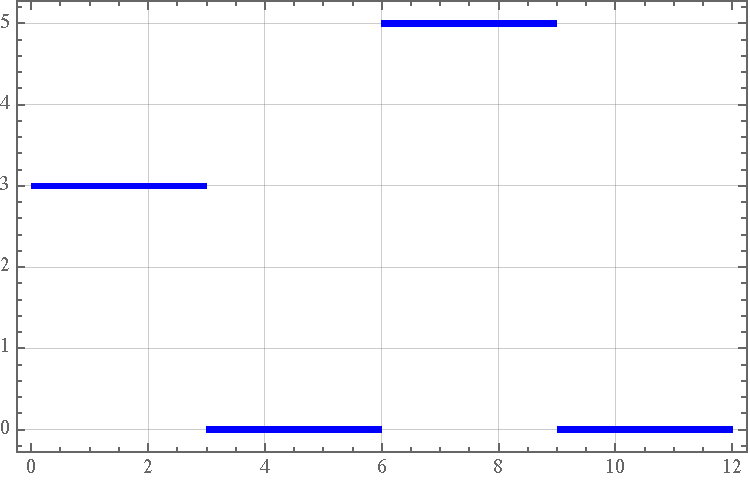
\includegraphics[width=0.45\textwidth]{images/exam/st_piecewise.pdf}
    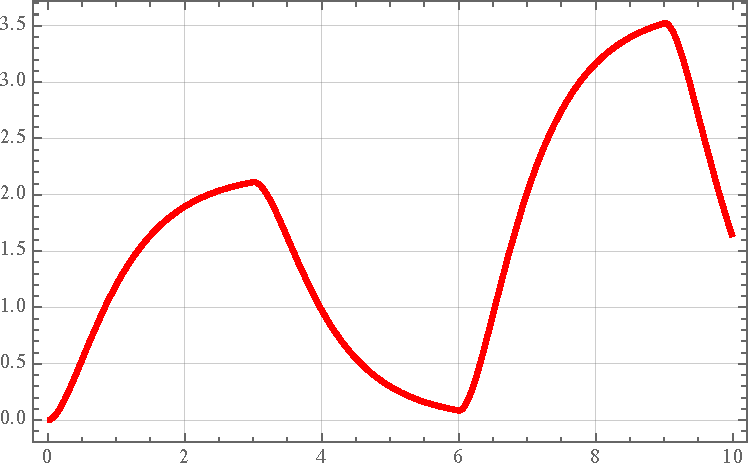
\includegraphics[width=0.45\textwidth]{images/exam/et_piecewise.pdf}
    \caption{Графіки для ступінчатого навантаження $\sigma(t)$ (зліва) та відповідне 
    розтягнення $\varepsilon(t)$ праворуч. Ми використали чисельні значення 
    $E_1=2.5$, $E_2=3.0$, $\mu_1=\mu_2=\mu_3=1.0$. Значення $\sigma(t)$ можна 
    побачити на графіку ліворуч. $\overline{\varepsilon} = (E_1+E_2)\sigma^*/E_1E_2 = 2.2$.}
    \label{fig:piecewise_2}
\end{figure}

\textcolor{purple}{\textbf{Графік для ступінчатого розтягнення.}} Розглянемо
наступне ступінчате розтягнення. Спочатку прикладемо розтягнення $\varepsilon^*$, потім
зменшимо його до нуля, знову прикладемо $\varepsilon^{**}$, а потім знову зменшимо до нуля.
Тоді розтягнення матиме вигляд:
\begin{equation*}
    \varepsilon(t) = \begin{cases}
        \varepsilon^*, & t < t^*, \\
        0, & t^* \leq t < t^{**}, \\
        \varepsilon^{**}, & t^{**} \leq t < t^{***}, \\
        0, & t \geq t^{***}.
    \end{cases}
\end{equation*}

Перший проміжок $t < t^*$ буде мати такий вигляд, як описано у ізометричному
експерименті (частина 3.1). Проміжки з нулем теж відповідають цьому випадку,
проте треба підставити $\varepsilon^* \equiv 0$. Зокрема, отримаємо залежність:
\begin{equation*}
    \sigma(t) = \sigma_Ce^{-t/T}, \quad \sigma(t^*) = \lim_{t \to t^*-0}\sigma(t)
\end{equation*}

Глянемо на результат на Рисунку \ref{fig:piecewise2}. Горизонтальна лінія: $\overline{\sigma} = E_1E_2 \varepsilon^*/(E_1+E_2)$.

% Draw two figures side by side using include
\begin{figure}[H]
    \centering
    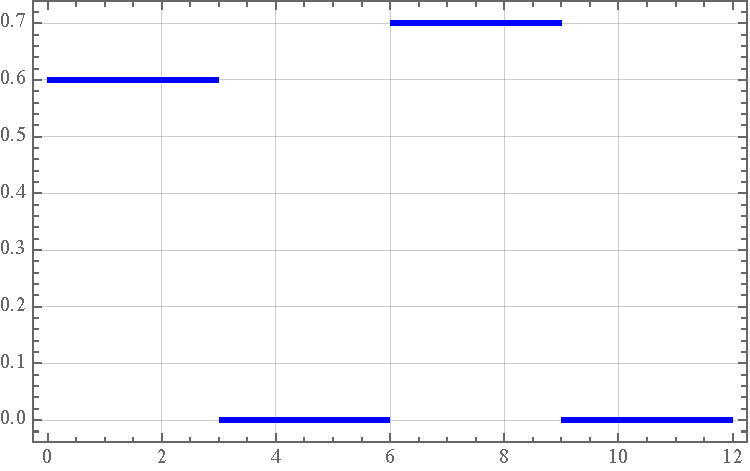
\includegraphics[width=0.45\textwidth]{images/exam/e_piecewise.pdf}
    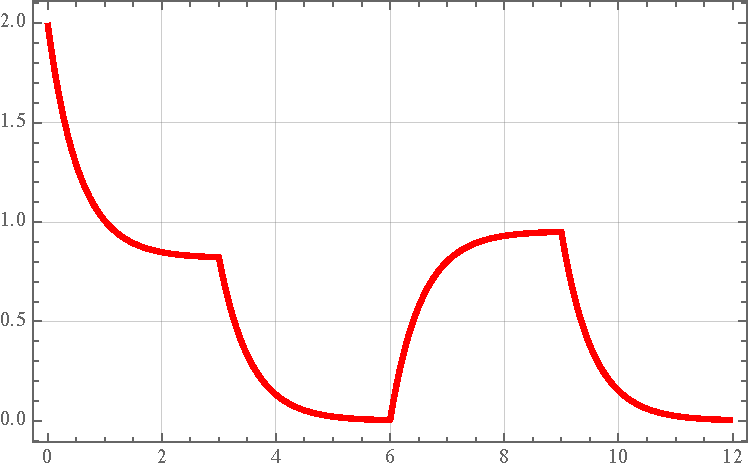
\includegraphics[width=0.45\textwidth]{images/exam/stress_piecewise.pdf}
    \caption{Графіки для ступінчатого розтягнення $\varepsilon(t)$ (зліва) та відповідне 
    навантаження $\sigma(t)$ праворуч. Ми використали чисельні значення 
    $E_1=2.5$, $E_2=3.0$, $\mu_1=\mu_2=\mu_3=1.0$. Значення $\varepsilon(t)$ можна 
    побачити на графіку ліворуч. На початку вважаємо $\sigma_0=2$. $\overline{\sigma} \approx 0.82.$}
    \label{fig:piecewise2}
\end{figure}

\textcolor{purple}{\textbf{Графік для динамічної поведінки.}} Тут графік
$\varepsilon(t)$ при початковій умові $\varepsilon(0) = \varepsilon_0
e^{i\varphi_0}$ та $\dot{\varepsilon}(0) = i\omega \varepsilon_0 e^{i\varphi_0}$ дасть
круг $|\varepsilon| = \varepsilon_0$ на комплексній площині. У випадку якщо
$\varepsilon_0$ або $\varphi_0$ підібрані неправильно, то рано чи пізно
траєкторія $\varepsilon(t)$ асимптотично вийде на коло $|\varepsilon| =
\varepsilon_0$, проте не одразу. Дивись Рисунок \ref{fig:complex}.

% Draw two figures side by side using include
\begin{figure}[H]
    \centering
    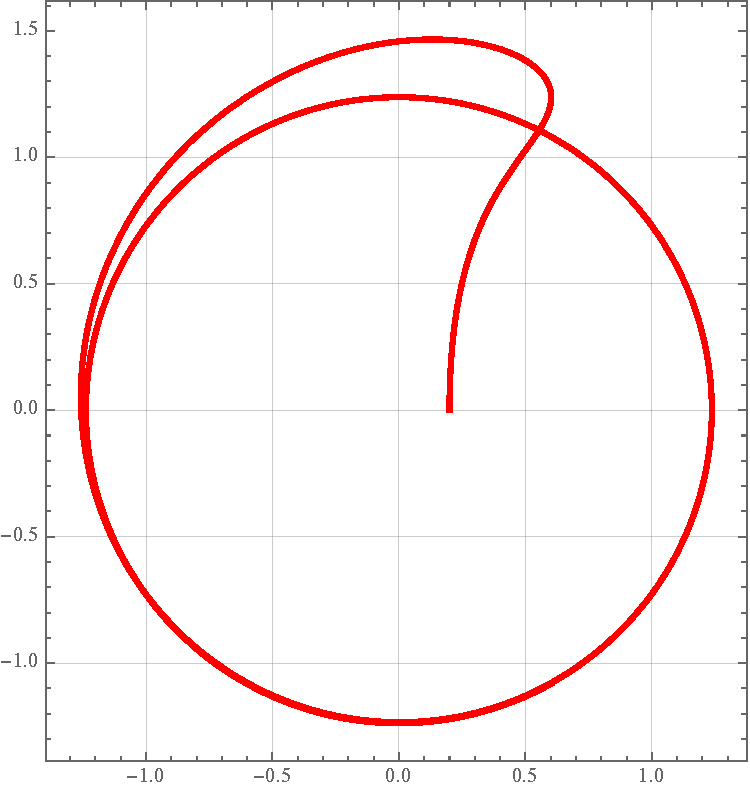
\includegraphics[width=0.45\textwidth]{images/exam/circle_wrong.pdf}
    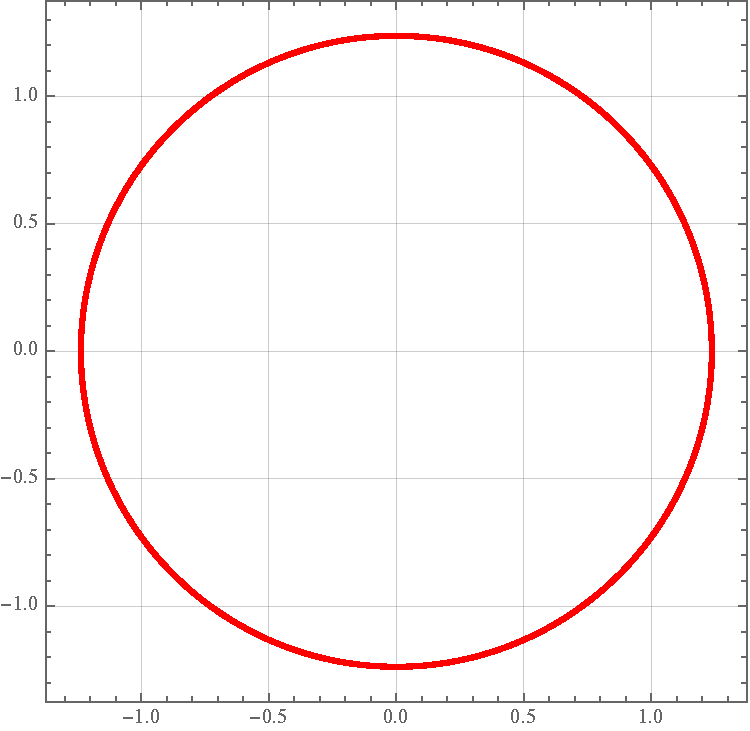
\includegraphics[width=0.45\textwidth]{images/exam/circle_correct.pdf}
    \caption{Графіки траєкторії $\varepsilon(t)$ для різних початкових умов.
    Параметри $E_1=2.5$, $E_2=3.0$, $\mu_1=\mu_2=\mu_3=1.0$, $\omega=1.0$,
    $\sigma^*=2.0$. Зліва показаний випадок початкової умови $\varepsilon(0)=0.2,
    \dot{\varepsilon}(0)=4i$. Праворуч початкова умова взята для $\varepsilon(0)=\varepsilon_0$, $\varepsilon(0)=i\omega \varepsilon_0 e^{i\varphi_0}$, де $\varepsilon_0 \approx 1.24$, $\varphi_0 \approx -0.497$.}
    \label{fig:complex}
\end{figure}


\textcolor{blue!90!white}{\textbf{Частина 4. Коментарі.}} Часто цю систему використовують 
для опису позвонка + міжпозвонкового диску. Вона описує як твердий біологічний матеріал
у вигляді хребця (позвонка), так і в'язкопружний матеріал у вигляді міжхребцевого диску.

\end{document}